\documentclass[12pt,a4paper,twocolumn]{article}
\usepackage{graphicx} % Required for inserting images
\usepackage{caption}
\captionsetup[figure]{font=small,labelfont=small}

\title{XELIS: A High-Performance BlockDAG for Private, Instant, and Scalable Decentralized Transactions and Applications}
\author{Xelis Team, Cyber Henry}
\date{October 2024}

\begin{document}

\maketitle

\section{Abstract}


XELIS is a private, scalable and fast Layer 1 blockchain based on BlockDAG technology, designed to ensure maximum user security and privacy for transactions and decentralized applications. While traditional public digital ledgers offer transparency, they often compromise user privacy by exposing wallet balances and transaction details. XELIS addresses this problem by offering a secure platform that combines advanced cryptographic techniques with an innovative data structure to preserve user privacy without sacrificing performance or scalability.\\

XELIS introduces a native utility coin that serves multiple purposes: it is used for transaction fees and network functions, acts as a medium of exchange, and serves as a store of value. This approach allows users to conduct fast, secure, and private transactions, deploy digital applications, and create decentralized financial services, all while maintaining the confidentiality of user balances and transaction amounts. XELIS ensures that while balances and transaction amounts are private, the relationship between sender addresses and receiver addresses is maintained within the public blockchain. This strategy ensures that compliance regulators and governmental officials are still able to track and locate wallets affiliated with potential fraudulent activities.\\

To achieve these goals, XELIS employs a BlockDAG architecture that merges concurrent chains instead of choosing between them, enhancing speed, scalability and security. It's complemented by homomorphic encryption using the Twisted ElGamal cryptosystem, using the Ristretto group over the popular elliptic curve 25519, enabling privacy for transaction amounts and balances while maintaining a high level of security. This encryption method relies on simple operations, such as addition and subtraction on ciphertexts only. As a result, the financial records of the blockchain's are manipulated solely in their encrypted state.\\

XELIS adopts an account-based model instead of the traditional UTXO model used by Bitcoin, resulting in a faster, more flexible, and smaller ledger that enhances privacy by eliminating the need to link inputs and outputs, thereby ensuring true fungibility. The platform supports a fast-sync feature that downloads only the latest state of the blockchain rather than its full history, further optimizing performance. Additionally, a pruning system can be employed to reduce blockchain size by removing old blocks and transactions.\\

A peer-to-peer (P2P) encrypted network ensures privacy by preventing traffic analysis, with all communication between nodes secured using ChaCha20-Poly1305 encryption, and keys are rotated frequently to enhance security. XELIS is also developing smart contracts and native XELIS VM (XVM) syntax to support the creation and deployment of decentralized applications and services, further expanding its ecosystem.\\

By combining these unique features, XELIS aims to provide a high-performance, secure, and privacy-focused blockchain platform that meets the growing demands of the digital economy while protecting user data and enabling seamless interactions.\\

\section{Introduction}

Cryptocurrencies have fundamentally changed the financial landscape by enabling decentralized and permissionless transactions on a global scale, all made possible by blockchain technology. However, this innovation faces significant challenges, particularly in balancing three essential aspects known as the “cryptocurrency trilemma”: decentralization, security, and scalability. Each of these pillars presents trade-offs that developers must navigate, as improving one often compromises the others.\\

The trilemma was popularized by Vitalik Buterin, highlighting the difficulty of optimizing all three properties simultaneously. Decentralization ensures that no single entity can control the system, enhancing resistance to censorship. However, increased decentralization may slow down consensus processes, which can affect overall performance. Security safeguards against fraud and attacks but often requires substantial computational resources, which can hinder performance if prioritized for speed. Scalability refers to a blockchain's ability to handle rising transaction volumes without sacrificing efficiency.\\

To complicate things further, XELIS introduces the concept of a quadrilemma or "quadlemma," as it will be referred to, adding privacy as a critical fourth pillar. As cryptocurrencies grow in adoption, concerns about transaction transparency and user confidentiality have become paramount. Privacy features allow users to engage in transactions without revealing sensitive information, yet achieving this can also affect scalability and decentralization. The quadlemma framework underscores the intricate balance required to develop effective blockchain solutions, highlighting the ongoing evolution in the field as developers seek to optimize all four pillars simultaneously without tradeoffs to the other pillars. \\




\begin{figure}
    \centering
    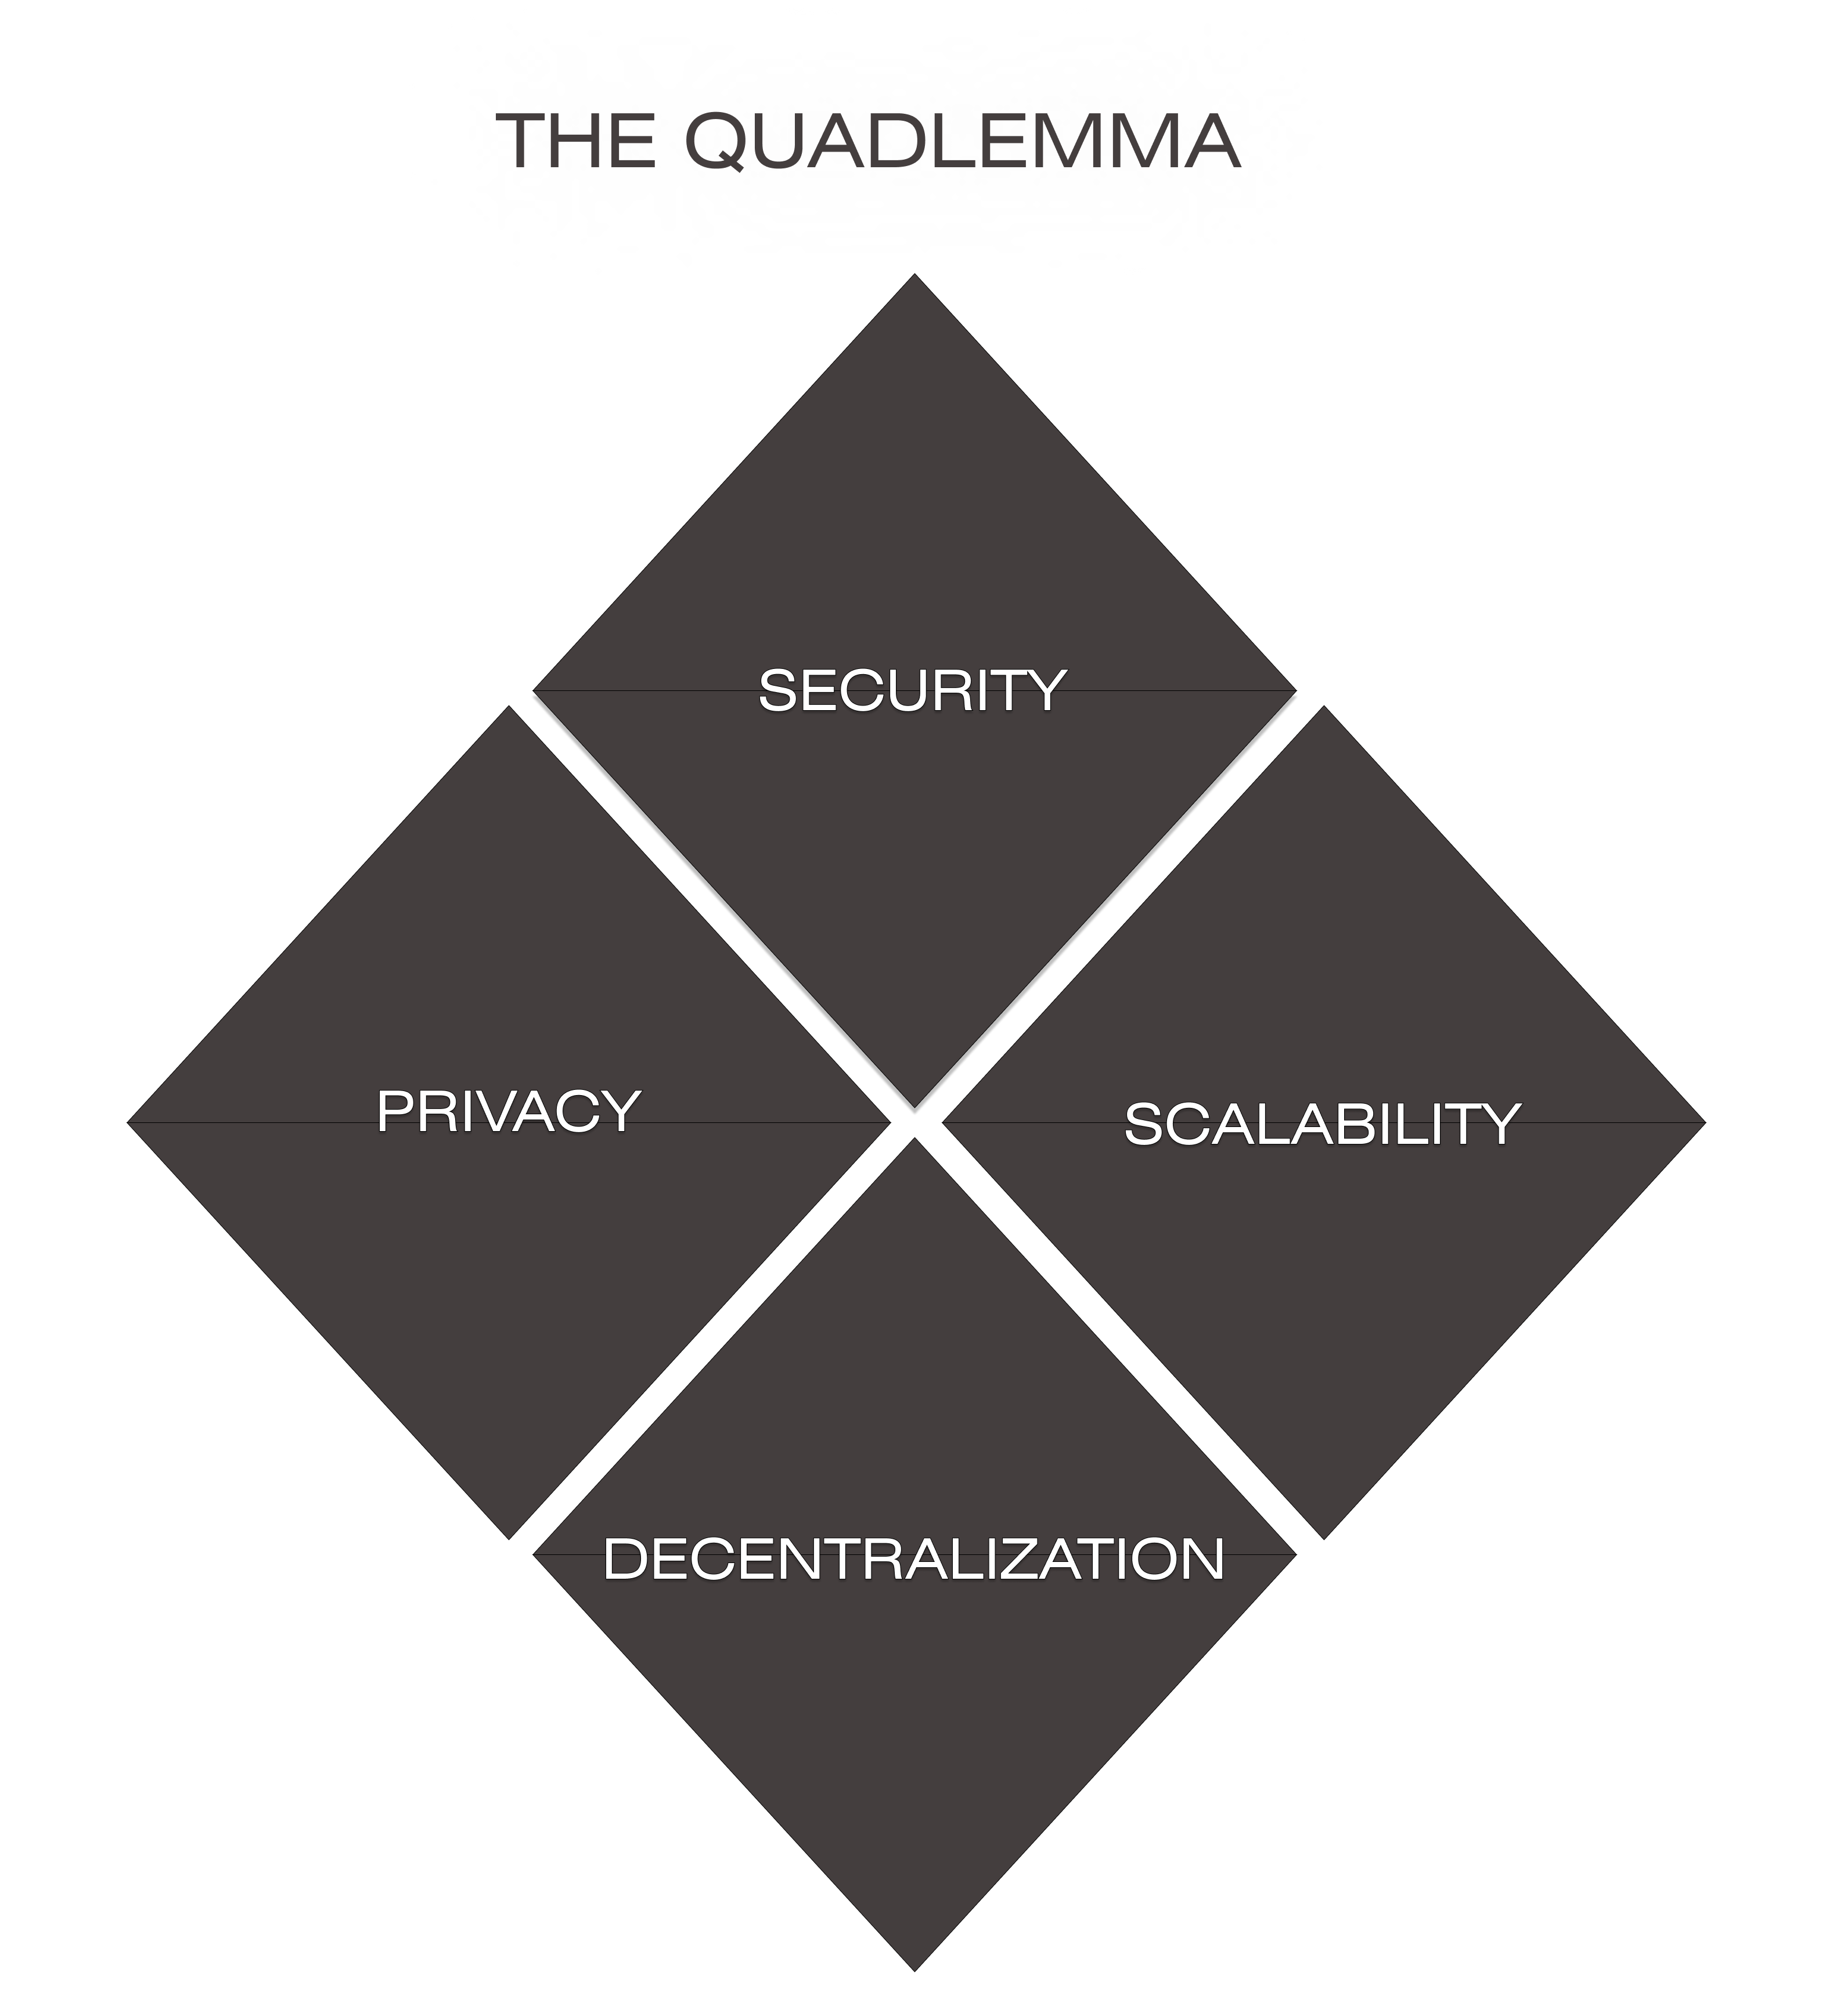
\includegraphics[width=1\linewidth]{Frame 9.png}
    \caption{Quadlemma, Cyber 2024}
\end{figure}

XELIS aims to address the quadlemma by integrating an ASIC-resistant Proof-of-Work consensus mechanism, advanced cryptographic techniques, and a blockDAG architecture. This approach ensures that decentralization, security, scalability, and privacy are all considered, positioning XELIS as a well-rounded cryptocurrency that does not compromise on any front. By embedding privacy features like homomorphic encryption and zero-knowledge proofs into its core, XELIS provides a platform that facilitates secure, confidential transactions while maintaining high performance and decentralization.\\

\subsection{BlockChain History}
The evolution of blockchain technology began with the invention of Bitcoin, progressing through various platforms and protocols, each with unique features and functionalities. While these platforms have significantly advanced decentralized technologies, they also have limitations that XELIS aims to address.\\

Bitcoin, introduced by Satoshi Nakamoto in 2008, was the first decentralized digital currency. Its primary innovation was the use of a distributed ledger known as blockchain, which enables secure, transparent, and immutable peer-to-peer transactions without a central authority. Key features include a Proof-of-Work (PoW) consensus mechanism, where miners compete to solve cryptographic puzzles, ensuring network security and transaction validation. The decentralization of Bitcoin, maintained by thousands of global nodes, contributes to its resistance to censorship. Furthermore, its fixed supply of 21 million coins creates a deflationary model. However, Bitcoin faces several limitations, including scalability issues, as it can only handle about seven transactions per second, making it unsuitable for high-volume applications. It also lacks smart contracts for programmable applications and has limited privacy, as transactions are pseudonymous yet publicly visible.\\

Ethereum, proposed by Vitalik Buterin in 2013 and launched in 2015, built upon Bitcoin’s foundation to introduce a more versatile platform capable of executing smart contracts. These self-executing contracts enable programmable decentralized applications (dApps) to run on the Ethereum blockchain. Key features include the Ethereum Virtual Machine (EVM), a Turing-complete environment for executing smart contracts, and a transition from PoW to a Proof-of-Stake (PoS) consensus mechanism in Ethereum 2.0, which aims to improve scalability and reduce energy consumption. Despite its innovations, Ethereum has scalability issues, supporting around 15 transactions per second, and experiences high transaction fees due to network congestion. Additionally, like Bitcoin, Ethereum transactions are publicly visible, limiting privacy.\\

Monero, launched in 2014, focuses on privacy and anonymity, offering enhanced features to protect users' transaction details and identities. It utilizes ring signatures to obscure the sender's identity by mixing their digital signature with others, employs stealth addresses for unique one-time transaction addresses, and incorporates Ring Confidential Transactions (RingCT) to keep transaction amounts private. However, Monero has scalability concerns due to larger transaction sizes, limited smart contract support, and regulatory scrutiny resulting from its full privacy focus.\\

Kaspa is a newer entrant, launched in 2021, designed to improve scalability and security using a BlockDAG (Directed Acyclic Graph) architecture. This allows multiple blocks to be mined and added concurrently, increasing throughput and reducing transaction confirmation times. Kaspa maintains high security and decentralization through its unique consensus algorithm, which is capable of handling higher transaction volumes. Despite these advantages, Kaspa lacks encryption and privacy features, making transaction details traceable, and it currently does not support smart contracts on Layer 1 for advanced decentralized applications and other financial services.\\


\subsection{Identifying the Gaps}

While Bitcoin, Ethereum, Monero, and Kaspa have each contributed significant advancement of blockchain technology, they also exhibit shortcomings. Bitcoin and Ethereum face scalability and privacy issues, with slow transaction times and high fees. Monero, while excellent for privacy, lacks scalability and smart contract functionality, limiting its broader adoption. Kaspa provides speed and scalability through its BlockDAG architecture but lacks the privacy features and Layer 1 programmability needed for a wider range of applications.\\

XELIS seeks to address these shortcomings and “Solve the quadlemma” by offering a next-generation Layer 1 blockchain that combines the best of each platform: security, high scalability and speed, robust privacy features, and a flexible environment for decentralized applications.\\

XELIS aims to create a secure, private, and easy to use environment that empowers users to engage in digital transactions and applications without compromise.\\


\subsection{The Risks of Public Ledger Transparency in Cryptocurrencies and the Case for XELIS}

While cryptocurrencies have transformed the financial landscape with their decentralized and digital alternatives, their reliance on public ledgers poses significant risks. Public blockchains, which record every transaction amount and wallet balance transparently, expose users and businesses to theft, fraud, social engineering, and privacy concerns. The visibility of wallet balances makes individuals vulnerable to targeted attacks and scams, while market participants may exploit the actions of large holders ("whales") to manipulate the market. These risks undermine the security and confidentiality of users, making it challenging for cryptocurrencies to serve as a safe medium of exchange.\\

XELIS offers a safer alternative by addressing these privacy shortcomings through innovative encryption mechanisms that protect wallet balances and transaction amounts. Unlike traditional cryptocurrencies, XELIS encrypts all wallet balances and transferred amounts, preventing public visibility and reducing exposure to fraud, social engineering, and market manipulation. By aligning with the privacy standards of traditional financial systems, XELIS ensures that users can conduct secure and private transactions, making it a practical choice for business and consumers everyday use. As the digital economy evolves, privacy-focused solutions like XELIS that preserve regulatory compliance by not privatizing addresses and identities will play a crucial role in safeguarding users and fostering broader adoption of cryptocurrencies.

\subsection{Main Objectives}

XELIS aims to provide enhanced confidentiality compared to Bitcoin, Ethereum and Kaspa by implementing encrypted balances and encrypted transaction amounts through the use of Homomorphic Encryption and Zero-Knowledge Proofs. This keeps the ledger decentralized while ensuring only the user has access to information about their holdings.\\

To achieve scalability and security, XELIS leverages a unique BlockDAG architecture and consensus mechanism. With a low block time target, the platform may encounter orphaned blocks, but the use of BlockDAG minimizes their occurrence while allowing for a higher block count, faster transaction confirmation, improved security, and increased transactions per second. To support the development of a comprehensive DeFi ecosystem, XELIS plans to introduce Smart Contract functionality through its proprietary Virtual Machine directly on the Layer 1 protocol. The platform will also allow the creation of Confidential Assets or fully decentralized tokens with the same level of privacy and decentralization as XELIS itself.\\

A decentralized network is essential for the security and resilience of the protocol eliminating single points of failure. XELIS achieves this by a wide distribution of nodes globally and utilizing an incentive based PoW algorithm that is friendly to both CPU and GPU miners, while remaining resistant to ASIC and FPGA hardware advantages.\\

Lastly, ease of use is a core focus of XELIS to drive widespread adoption for everyday use. This focus extends not only to end-users but also to developers, providing them with the tools and support needed to create and integrate diverse applications seamlessly.\\

\section{Technology and Architecture}

This section provides an overview of the Xelis technology and architecture, which is designed for high performance. Xelis enables fast transaction and processing speeds, ensuring responsiveness even during peak usage. Its scalable architecture supports growth while maintaining system integrity, and it incorporates robust security and state-of-the-art encryption methods to ensure user privacy. This combination of features positions Xelis as a practical solution for the demands of decentralized applications and financial systems.\\

\subsection{High Speed and Scalable BlockDAG Architecture}

A BlockDAG (Directed Acyclic Graph) is an advanced data structure used in blockchain technology that differs significantly from traditional linear blockchain designs. Unlike a conventional blockchain where blocks are added in a single linear sequence, a BlockDAG allows multiple blocks to be created and accepted simultaneously, even at the same height. This parallel structure enhances scalability by enabling a higher volume of transactions and faster confirmation times, while also reducing the risk of centralization by providing flexibility in block addition.\\

\begin{figure}
    \centering
    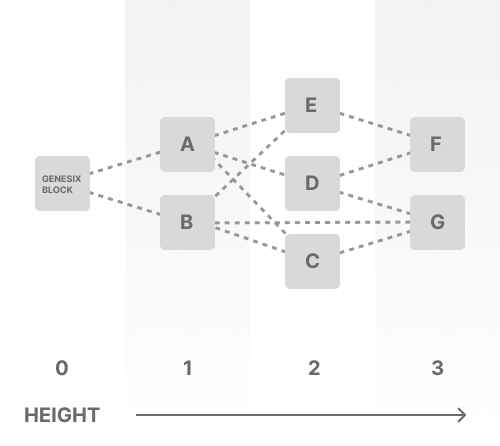
\includegraphics[width=0.8\linewidth]{Frame 1 (7).png}
    \caption{BlockDAG, Xelis Team 2024}
\end{figure}


\subsubsection{Topological Order}

BlockDAG needs to generate a deterministic order to execute all the blocks and transactions in the same way across all nodes to keep the compatibility and exact state in the network. \\

XELIS uses a topological order, where blocks are assigned a "topological height" (or "topo-height") based on their position within the DAG. This topological order is crucial for establishing a consistent and deterministic sequence for the blocks, making the relationships within the DAG clear. Blocks with a greater topo-height are considered later in the order. This dynamic approach means that the topological height can be adjusted during reorganizations until it reaches a point known as the "stable height." When multiple branches exist within the DAG, the order is determined by the cumulative difficulty (the total difficulty sum of all block tips), ensuring that the block with the highest cumulative difficulty is prioritized.\\

Topological order ensures that for every directed edge (u, v) in the DAG, node u precedes node v in the sequence, effectively representing dependencies and maintaining the correct execution order without creating cycles. This systematic arrangement allows for reorganization within the DAG while preventing deep reorganization attacks by dishonest actors, as blocks below the stable height are fixed and cannot be altered.\\

\subsubsection{Stable Height}

The stable height in XELIS BlockDAG design represents a point in the chain beyond which block a DAG reorganization is not allowed, ensuring the integrity and security of the blockchain. Blocks below this height are immutable, safeguarding the chain from deep reorganizations by malicious entities attempting to inject older blocks. The stable height is typically set to a minimum of 8 blocks from the current top of the main chain, providing a secure buffer zone that prevents attacks and maintains consistency.

\subsubsection{Block Types in the BlockDAG}

XELIS utilizes four different types of blocks within its BlockDAG architecture, each serving a specific function:\\

\textbf{Side Block:} A side block is created when a block loses the race against another block at the same or lower height. Side blocks are ordered and executed in the chain but receive only 30 percent of the expected block reward. Transactions within side blocks are verified and executed if they have not already been processed.\\

Example:
If Block A is ordered at topo-height 100 with a height of 95, and Block B is ordered at topoheight 99 with a height of 96, then Block A becomes a side block.\\

\textbf{Sync Block:} A sync block must be the only block at its height within the stable height and must have the highest cumulative difficulty compared to other blocks within the recent stable limit. Sync blocks are mandatory for maintaining chain consistency.\\

\textbf{Normal Block:} A normal block is any block that is neither a side block nor a sync block. It is ordered and executed according to standard BlockDAG rules.\\

\textbf{Orphaned Block:} A block becomes orphaned if it fails to meet the difficulty requirements or deviates from the main chain. Orphaned blocks are excluded from transaction processing, and no rewards are granted to their miners. They are also not shared during a chain-sync with other peers as they are not part of the consensus.

\subsubsection{Consensus Rules and Handling of Transactions}

In the XELIS BlockDAG, multiple blocks may exist at the same height, allowing up to three previous block hashes per block. During the Proof of Work (PoW) process, the three heaviest tips (blocks) are selected as references. These tips must not differ by more than 9 percent in difficulty to ensure fairness. Transactions can appear in multiple blocks if they do not share the same tip branch, and the client protocol ensures that each transaction is executed only once.\\

The circulating supply and miner rewards are calculated based on the topological height, which is recomputed whenever the topoheight changes. Transactions are processed in topological order and can be re-verified or re-computed during reorganizations. The "longest chain" rule, as used in traditional blockchains, is maintained by selecting the chain with the highest cumulative difficulty in cases of branch conflicts.\\

The cumulative difficulty is the total work being done from the genesis block to the latest block in the chain, following the topological order. As an example, blockchain A may be longer in height than blockchain B, but A will not be selected, because B has side-blocks which increase the cumulative work and have a longer topological height.\\

This approach enhances the scalability, security, and flexibility of the XELIS network, allowing for more efficient processing and higher throughput while maintaining the decentralized principles of blockchain technology.\\

\subsection{Enhancing Privacy with Homomorphic Encryption}

Homomorphic Encryption (HE) is a powerful cryptographic technique that enables computation on encrypted data without the need for decryption. This means that operations can be performed directly on encrypted data, and the results, when decrypted, will reflect the outcome of the same operations if they had been carried out on the original, unencrypted data. The primary goal of Homomorphic Encryption is to preserve the confidentiality of data while still allowing for meaningful operations to be conducted on it.\\

In the context of XELIS transactions and account management, Homomorphic Encryption significantly enhances privacy. By ensuring that all operations are performed on encrypted values, XELIS maintains the confidentiality of account balances and transaction amounts. This means that only the involved parties can access the actual values, safeguarding user privacy against any unauthorized observers.\\

\subsubsection{The Role of ElGamal in XELIS}

ElGamal Encryption, named after its inventor Taher Elgamal, is a public-key cryptosystem founded on the difficulty of computing discrete logarithms. Introduced in 1985, it provides a robust framework for encryption that is well-suited for various applications. In the XELIS ecosystem, an implementation of the ElGamal cryptosystem is utilized to leverage its homomorphic properties.

XELIS specifically employs a variant known as Twisted ElGamal. This adaptation integrates Pedersen commitments into every ciphertext, enhancing compatibility with Bulletproofs—a tool for transaction verification that accelerates the verification process. Despite these modifications, Twisted ElGamal retains the same homomorphic properties and security guarantees as the original ElGamal system.\\

\subsubsection{Homomorphic Properties of ElGamal}

ElGamal Homomorphic Encryption boasts several key properties,\\

\textbf{Additive Property:} If you have two ciphertexts, c1 and c2, that encrypt messages m1 and m2 respectively, you can compute a new ciphertext c3 that encrypts the sum m1 + m2 without needing to decrypt c1 and c2.\\

\textbf{Multiplicative Property:} Given a ciphertext c1 that encrypts a message m1 and a plaintext m2, you can compute a new ciphertext c2 that encrypts the product m1 * m2 without decrypting c1.\\

\textbf{Subtractive Property:} If you have two ciphertexts, c1 and c2, encrypting messages m1 and m2 respectively, you can produce a new ciphertext c3 that encrypts the difference m1 - m2 without decrypting c1 and c2.

For XELIS's protocol, only the additive and subtractive properties are utilized. Addition is used to increment a receiver's balance, while subtraction is used to decrement a sender's balance. Multiplication is not necessary for the typical blockchain operations performed by XELIS, as it primarily involves transferring exact values between accounts.\\ 

The following section will discuss why a modified version of ElGamal has been chosen for XELIS

\subsubsection{Why Choose Twisted ElGamal}

Twisted ElGamal stands out due to its robust security and compatibility with the curve25519 curve, which is implemented in XELIS through Ristretto Points. Its homomorphic properties make it an ideal choice for the XELIS protocol. Unlike Fully Homomorphic Encryption (FHE) schemes, which, while highly versatile, are often slow and involve significant computational overhead due to the growth in ciphertext size with each operation, ElGamal’s operations maintain a consistent ciphertext size. This stability makes ElGamal more suitable for XELIS, where only basic arithmetic operations are required.\\

In contrast, FHE schemes typically introduce additional "noise" that enlarges ciphertexts with every operation, complicating their use in applications like XELIS that demand efficient and scalable encryption.\\

\begin{figure}
    \centering
    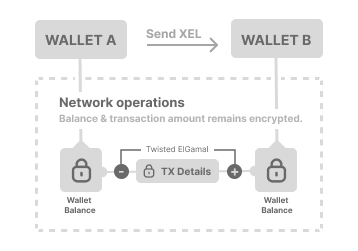
\includegraphics[width=0.9\linewidth]{ElGamal Homomorphic XEL (1).png}
    \caption{Twisted Elgamal, Xelis Team 2024}
    \label{fig:enter-label}
\end{figure}


\subsubsection{Twisted ElGamal and BlockDAG Integration}

In addition to the cryptographic techniques discussed, XELIS incorporates a BlockDAG architecture, which complements its privacy-enhancing measures by providing a scalable and efficient framework for transaction processing. The BlockDAG structure supports high transaction throughput and quick validation, aligning well with XELIS’s homomorphic encryption.\\

Overall, the integration of ElGamal encryption with Homomorphic Encryption and BlockDAG architecture ensures that XELIS provides a secure, private, and efficient transaction environment for its users.\\

\subsection{Deciphering Transactions with Zero-Knowledge Proofs}

Zero-Knowledge Proofs (ZKPs) are a sophisticated cryptographic method enabling one party, known as the prover, to convincingly demonstrate knowledge of a specific piece of information to another party, called the verifier, without disclosing the actual information itself. This technique ensures that the verifier can be confident in the prover's knowledge while maintaining the confidentiality of the information.\\

In the context of XELIS, zero-knowledge proofs are crucial for validating transactions involving encrypted data. Specifically, XELIS employs ZKPs to confirm the validity of ciphertexts—encrypted representations of transferred amounts. The verification process involves two critical checks:\\

\textbf{Range Verification:} Ensures that the transferred amount represented by the ciphertext does not exceed the encrypted balance held by the sender.\\

\textbf{Non-Negativity Verification:} Confirms that the ciphertext represents a non-negative value.
To perform these verifications, XELIS utilizes Bulletproofs, a cutting-edge zero-knowledge proof protocol that is both non-interactive and does not require a trusted setup. Bulletproofs facilitate efficient range proofs, which are essential for confirming the validity of encrypted amounts. XELIS is also aggregating range proofs to achieve faster verification times, with a target of under 1 millisecond per transaction.\\

\subsubsection{Optimizations for Efficiency}

To handle the scalability and efficiency of transaction verification, XELIS incorporates several optimizations:\\

\textbf{Batching and Aggregation:} Transactions are grouped together to streamline the verification process. By batching and aggregating Range Proofs and Sigma Proofs, XELIS significantly reduces the time required for verification.\\

\textbf{Source Commitment:} XELIS groups the sum of spent assets into a single source commitment per asset. This approach decreases the need to update the sender's balance multiple times in a single transaction, thereby enhancing performance.\\

\textbf{Additional Potential Optimizations:} Future improvements may include reducing the frequency of key and ciphertext compression/decompression during verification and employing pre-computed scalar bases for more efficient validation.\\

By performing these optimizations, verifying 100 transactions takes approximately 0.40 milliseconds per transaction, leading to a block verification time of around 40 milliseconds. This throughput translates to the potential handling of up to 2,500 transactions per second.

\subsubsection{Addressing Front Running and Transaction Order}

Front Running concerns arise from the need to base range proofs on the current encrypted balance during transaction creation. The integration of balances in transactions can lead to potential issues,\\

\textbf{BlockDAG and Transaction Order:} In XELIS's BlockDAG architecture, blocks are not strictly ordered by height but by their cumulative difficulty, allowing for potential reordering of transactions. This can affect transactions if their execution order changes, resulting in a transaction that might get orphaned. However, XELIS’s use of block TIPS (previous block hashes a block is based on) ensures that transactions within the same branch are processed in the correct order and are thus valid.\\

\textbf{Incoming Transactions:} If a user's transaction is preceded by another transaction, the first user’s zero-knowledge proof may become outdated. To address this, XELIS verifies transactions based on the most recent balance from the last outgoing transaction, ensuring validity even if incoming transactions occur between proof creation and execution.\\

\textbf{Outgoing Transactions:} The order of outgoing transactions must be preserved to maintain balance validity during proof verification. XELIS uses an incrementing nonce to prevent replay attacks and ensure that transactions follow the same sequence as when the ZKP was created.
Handling Multiple Transactions: When multiple transactions are involved, XELIS distinguishes between Output Balances (current balance minus outputs spent) and Final Balances (real user balance with all incoming and outgoing funds). ZKPs are created using the final balance, but for cases involving multiple outputs split by incoming transactions, the output balance is used for verification. The system maintains the output balance as an internal process, ensuring future transactions remain valid based on the chain state.\\

\subsection{XELIS Elliptic Curve Discrete Logarithm Problem}

The Elliptic Curve Discrete Logarithm Problem (ECDLP) is a cornerstone of elliptic curve cryptography (ECC), a widely used cryptographic system renowned for its security and efficiency. The ECDLP forms the basis of ECC's security, relying on the computational difficulty of solving a specific mathematical problem.\\

ECDLP involves finding the exponent k in the equation Q = k * P, where P is a point on an elliptic curve, Q is the result of multiplying P by k. The difficulty lies in finding the private key k when only the public key Q and the base point P are known.\\

For traditional discrete logarithm problems, such as those in finite field-based systems like RSA or Diffie-Hellman, the best-known algorithms have exponential time complexity, making them computationally infeasible for large key sizes. Similarly, the ECDLP is believed to be hard, but it is computationally more efficient compared to its finite field counterparts for equivalent security levels. This efficiency makes elliptic curve cryptography attractive for resource-constrained environments, such as mobile devices and IoT devices.\\

\subsubsection{Fast Algorithm for Solving ECDLP}

To solve the ECDLP efficiently, XELIS uses advanced algorithms such as Baby Step Giant Step (BSGS). This algorithm provides a practical approach to solving the ECDLP by reducing the problem to a manageable size. The BSGS algorithm involves creating two tables to help decode an integer representing a point on the elliptic curve. \\

Only approximately 330 MB of precomputed tables with L1 = 26 are needed to solve the ECDLP for any point in the curve in a few milliseconds to decode an integer up to \(2^{48}\).\\

The overview of BSGS goes as follows:\\

Our target point, which we want to decode, represents an integer in the range \([0, 2^{(L1 + L2)}]\).\\

We have a T1 hash table, where the key is the curve point and value is the decoded point. \(T1 = <i * G => i | i\) in \([1, 2^{L1}]>\)\\

We have a T2 linear table (an array), where T2 = \([j * 2^{L1} * G |\) j in \([1, 2^{L2}]]\)
For each j in \(0..2^{L2}\)\\

Compute the difference between \(T2[j]\) and the target point.\\

If we have an occurrence in T1 table, the decoded integer is \(j * 2^{L1} + i\).\\

\subsubsection{Optimizations for Enhanced Performance}

In XELIS, the regular BSGS algorithm is further improved with several optimizations,\\

\textbf{Batching Techniques:} Instead of using a tree-based Montgomery trick, we employ batched inversion, which is implemented in FieldElement. This method improves computational speed.\\

\textbf{Table Optimization:}Reduced Storage, Table T1 only contains the truncated x coordinates.\\

\textbf{Efficient Hashing:} Cuckoo hashing is used, with hash values directly derived from a subset of the bytes of the point.\\

\textbf{Affine Coordinates:} For efficient point addition, we use affine Montgomery coordinates, which require fewer modular inversions compared to Edwards coordinates.\\

\textbf{Input Shifting:} By leveraging the property −(x,y)=(x,−y) on the Montgomery curve, we reduce the need for storage and inversions by half.\\

\textbf{Fixed Constant:}The L2 constant is fixed to only ~16 kB tp simplify processing and ensure manageable table sizes. It would require slightly more modular inversions but has no visible impact on performance and can save more than 100 MB on disk in some cases.\\

It is important to note that we are dealing with a curve which has cofactors. To handle curves with cofactors, we need to multiply by the cofactor before running the ECDLP to ensure a canonical encoding of curve points.\\

\subsubsection{ECDLP Summary}

The ECDLP is a fundamental problem underpinning the security of elliptic curve cryptography. ECC’s efficiency compared to traditional cryptographic systems makes it highly suitable for constrained environments. The Baby Step Giant Step algorithm, with its associated optimizations, provides a fast and effective means of solving the ECDLP, enhancing ECC's practical applicability and security. Through precomputed tables, efficient hashing, and optimized algorithms, XELIS ensures rapid and reliable cryptographic operations within a secure framework.\\

This implementation is only used in the wallet to decode balances and transaction amounts in the most efficient way when required.

\subsection{Account Model vs. UTXO Model}

XELIS operates on an account model architecture, a framework that differs from other cryptographic systems and blockchain architectures. Among the most common models used to manage and track transactions are the Account Model and the UTXO (Unspent Transaction Output) Model. Each of these models offers its own unique advantages, functionalities and use cases, affecting aspects like performance, privacy, and ease of use.\\

\subsubsection{UTXO Model}

The UTXO Model is the foundational structure used by Bitcoin and several other cryptocurrencies. The model works as followed,\\

\begin{itemize}
    \item \textbf{Unspent Transaction Outputs (UTXOs):} The system tracks discrete pieces of value called UTXOs. Each UTXO represents a specific amount of cryptocurrency that has not yet been spent.\\
    
    \item \textbf{Transaction Inputs and Outputs:} To spend cryptocurrency, a transaction references one or more UTXOs as inputs and creates new UTXOs as outputs. This ensures that value is always accounted for and that there is no double spending.\\
   
\begin{figure}
\centering
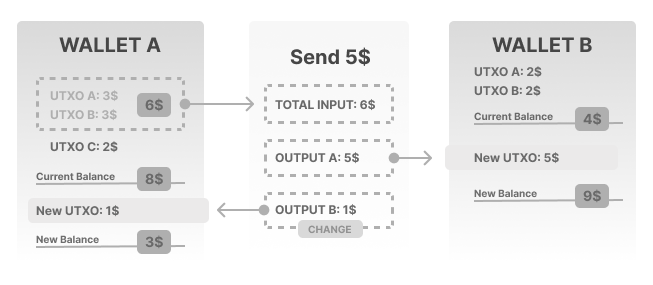
\includegraphics[width=1\linewidth]{Frame 1 (8).png}
\caption{UTXO Model, Xelis Team 2024}
\end{figure}
  
    \item \textbf{State Reconstruction:} The current state of a user's balance is derived by scanning through all transactions and summing the UTXOs associated with their addresses. This process can be resource-intensive, especially as the blockchain grows.\\
\end{itemize}

\textbf{Advantages of UTXO,}\\
\begin{itemize}
\item \textbf{Immutability:} UTXOs are immutable once created, making the system resilient to certain types of errors and attacks.\\ 

\item \textbf{Transparency:} Each transaction’s UTXOs can be individually verified, contributing to the system's overall security and transparency.\\
\end{itemize}
\textbf{Disadvantages of UTXO,}\\ 
\begin{itemize}
\item \textbf{Complexity:} Managing and reconstructing the state of an account from UTXOs can be computationally demanding and complex.\\ 

\item \textbf{Privacy Concerns:} Linking inputs and outputs can potentially expose spending patterns and transaction details, impacting user privacy.\\
\end{itemize}
\begin{figure}
    \centering
    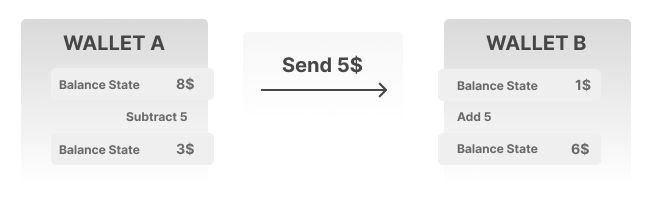
\includegraphics[width=0.9\linewidth]{Frame 2.png}
    \caption{Account Model, Xelis Team 2024}
\end{figure}

\subsubsection{Account Model}

The Account Model, employed by Ethereum and some other blockchains, represents a different approach to managing transactions and balances. The model works as followed,\\

\begin{itemize}
    \item \textbf{Accounts:} In this model, each account has a balance and state associated with it. Transactions update the balance of these accounts directly.\\
    
    \item \textbf{State Changes:} When a transaction is processed, it modifies the state of the involved accounts by deducting from one account and adding to another.\\
    
    \item \textbf{Simplified State Management:} Instead of tracking individual UTXOs, the system maintains the current state of each account, making it easier to determine balances and process transactions.\\
\end{itemize}

\textbf{Advantages of Account Model,} \\
\begin{itemize}
\item \textbf{Efficiency:} The Account Model simplifies transaction processing by directly updating account balances, leading to faster and more efficient state management.\\

\item \textbf{Flexibility:} It supports more complex transactions and smart contracts, enabling a broader range of functionalities compared to the UTXO Model.\\

\item \textbf{Privacy:} Since the model does not link inputs and outputs, it provides enhanced privacy and fungibility. This separation reduces the risk of transaction analysis revealing spending patterns or amounts.\\

\item \textbf{Balance:} no need to scan the whole chain to find the most up-to-date balance, you can get the latest state of an account in one request and is independent of the chain size.\\
\end{itemize}
\textbf{Disadvantages,} \\
\begin{itemize}
\item \textbf{State Size:} While more efficient for processing, the system needs to maintain the current state of all accounts. 

\item \textbf{Complexity in Implementation:} Implementing smart contracts and maintaining the integrity of account states require sophisticated mechanisms.\\
\end{itemize}
\subsubsection{Why the Account Model was Chosen for XELIS}

XELIS has adopted the Account Model instead of the UTXO Model for several compelling reasons:
Performance: The Account Model allows for faster transaction processing. By directly updating account balances, XELIS minimizes the computational overhead involved in tracking and managing discrete UTXOs. This efficiency is particularly advantageous for handling high transaction volumes and ensuring swift processing.\\
\begin{itemize}
\item \textbf{State Size and Syncing:} The Account Model facilitates a more streamlined approach to state management. With the ability to maintain and download only the current state of the blockchain, XELIS supports a fast-sync feature. This approach significantly reduces the amount of historical data that needs to be downloaded, enhancing the speed and ease of synchronization for new nodes.\\

\item \textbf{Flexibility and Privacy:} The Account Model offers a more flexible framework for implementing complex transactions and smart contracts. Additionally, it improves privacy by eliminating the need to link transaction inputs and outputs. This separation helps ensure greater fungibility of assets.\\

\item \textbf{Ease of Use:} For users and developers, the Account Model provides a more intuitive system. It simplifies the process of managing and tracking balances without the need to handle discrete UTXOs, making the overall experience more user-friendly.\\
\end{itemize}
In summary, while the UTXO Model has its merits, particularly in terms of security and transparency, the Account Model's advantages in performance, flexibility, and privacy make it a preferable choice for XELIS. By leveraging the Account Model, XELIS aims to provide a more efficient, user-friendly, and private blockchain experience.\\

\subsection{Proof of Work}

In the realm of blockchain technology, ensuring the security and integrity of decentralized networks is paramount. One of the foundational mechanisms for achieving this is Proof of Work (PoW). PoW is a consensus algorithm that underpins the security and operational efficacy of many blockchain systems, most notably Bitcoin. At its core, PoW is designed to address the challenges of trust and coordination in a decentralized network by requiring participants, or miners, to solve complex computational problems.\\

In the XELIS network, Proof of Work serves as the bedrock for achieving consensus and validating transactions. This section delves into the principles behind XELIS’ PoW, its implementation within the XELIS framework, and how it contributes to the robustness and decentralization of our blockchain ecosystem.\\

\subsubsection{Decentralized Vision of XELIS Mining:}

At XELIS, we envision a decentralized mining future that maximizes equal participation by prioritizing CPUs and GPUs, which are accessible to all. By limiting the performance of specialized hardware like FPGAs and ASICs, we aim to reduce centralization risks and ensure a more equitable distribution of mining rewards. Our commitment is to foster an inclusive ecosystem where individuals from diverse backgrounds can actively contribute to the network, enhancing both its security and community spirit.\\

To accomplish our vision, we’ve built our own PoW hashing algorithm that is fully compatible with GPUs and CPUs while reducing the advantages of ASICs and FPGAs. This is made possible by utilizing an algorithm which requires high amounts of memory bandwidth, as memory bandwidth is what most hardware becomes bottlenecked on. A fixed-size scratchpad is generated for each hash based on the hashed input to prevent any input attacks. Scratchpad must be the most distributed possible in order to prevent any patterns that could be leveraged to gain unfair advantages. It is based on the popular ChaCha8.\\

All inner hashing and final output hash are based on Blake3 algorithm to be really fast and provide a good-quality hash. The hash generation should be as fast as possible for fast PoW verification when a block is verified.\\

\subsection{Difficulty Adjustment Algorithm}

The difficulty adjustment algorithm is a fundamental aspect of any blockchain protocol utilizing a Proof-of-Work (PoW) consensus mechanism. Its primary role is to ensure that the time between new blocks remains close to a predefined target, even as the network’s hashing power varies. By stabilizing the block generation rate, this mechanism is essential for maintaining consistent issuance of new coins and enhancing the overall security of the network.\\

The cost of attacking a blockchain network is directly proportional to its hashing power. Therefore, networks with significant hashing power distributed across numerous participants are inherently more secure against malicious activities. Consequently, an efficient difficulty adjustment algorithm is critical for preserving both the security and stability of the network.\\

\subsubsection{XELIS Difficulty Adjustment Algorithm}

XELIS employs a streamlined version of the Kalman Filter to accurately estimate the network’s hash rate based on the frequency of incoming blocks. This sophisticated estimation is pivotal for dynamically adjusting the difficulty target for each new block. The Kalman Filter is a mathematical algorithm used for estimating the state of a dynamic system from a series of noisy measurements. It works through a recursive process that combines predictions from a system model with actual measurements to produce accurate estimates. By applying a prediction-update cycle, the filter minimizes the variance of estimation errors and adapts to new data in real time. This technique is widely utilized in fields such as navigation, robotics, and finance to track and predict system states amidst uncertainty and noise.\\

The Kalman Filter offers a notable advantage by quickly converging on the true network hash rate and effectively mitigating the impact of transient hash rate fluctuations. This capability ensures that the difficulty adjustments are both timely and accurate.\\

In XELIS, the difficulty adjustment occurs at every block. The algorithm utilizes the heaviest block’s tip as the reference point for determining the parent difficulty. This reference is selected based on the cumulative difficulty within its Directed Acyclic Graph (DAG) branch, which informs the difficulty parameter for the subsequent block.\\

To estimate the time required to solve a block, the algorithm employs the timestamp from the tip of the most recent block available. This selection is based on the highest timestamp among all block tips, which serves as the basis for the parent timestamp parameter. The time to solve the current block is then approximated by subtracting the timestamp of the current block from this reference timestamp.\\

By integrating these methods, XELIS ensures that its difficulty adjustment mechanism remains robust and responsive, effectively balancing network performance and security.

\subsection{Client Protocol}

The Client Protocol is a specialized feature designed to support BlockDAG architecture, allowing for advanced transaction handling in a decentralized network. Unlike traditional blockchain systems, where a transaction included in multiple blocks might be rejected to prevent double spending, the Client Protocol in a BlockDAG framework accommodates such scenarios by accepting all relevant blocks and resolving double spending issues through a systematic approach.\\

In this protocol, transactions are processed based on their topological order within the BlockDAG. For example, if Block A, at topo-height 1000, serves as the common base tip for two subsequent blocks, Block B and Block C—both at same height containing the same transaction, T1—the Client Protocol will prioritize and execute transaction T1 from Block B, assuming it is the first in the topological order. The protocol ensures that the transaction is executed only once by marking it as executed and by considering the previous tips of the block candidate to prevent duplication during branch merges.\\

\subsection{Transaction Fees}

The XELIS network incorporates a robust fee structure to manage transaction costs, reward miners, and mitigate spam attacks. Transaction fees are exclusively payable using the native XELIS asset and are determined by several factors, \textit{Size in Bytes:} A fee of 0.0001 XELIS is applied per 1024 bytes of transaction data. This fee structure helps to control chain bloating and manage disk usage.
\textit{Transfer Count: }Each transfer within a transaction incurs an additional fee of 0.00005 XELIS, reflecting the computational effort required for Homomorphic Encryption. More transfers necessitate additional computation and verification. \textit{Newly Created Addresses:} A one-time fee of 0.001 XELIS is charged for registering new addresses. This fee is designed to prevent spamming attacks by ensuring that each new address incurs a cost, thus avoiding the creation of numerous fake or unused accounts. This registration fee can be fulfilled either through mining or receiving a transaction.\\

\subsection{Extra Data Transfer Capabilities}

XELIS not only facilitates transactions but also supports data transfer with strong encryption. Data stored on the blockchain can be shared or kept private, with integration options allowing for encrypted data to be included in transactions. Each transaction supports up to 32 KiB of encrypted data (maximum 1 KiB per transfer), which can be easily manipulated using JSON encoding and decoding.\\

Encrypted data within a transaction is injected into the extra\_data field, enabling a variety of applications from sending private messages and managing deposits to including shipping information and providing proofs of transactions. However, this data inclusion is limited in size to prevent excessive chain growth. Users must trust the service providers for executing requested actions, as the protocol does not ensure automatic execution.\\

\subsection{Integrated Addresses}

XELIS provides a feature known as integrated addresses, which combine wallet addresses with additional embedded data, similar to Monero's payment IDs but with broader functionality. Integrated addresses allow users to include various types of data directly within the address, facilitating unique uses such as identifying deposits, including shipping information, or sending messages.\\
\begin{itemize}
\item \textbf{How It Works:} When sending a transaction to an integrated address, the wallet encrypts the data and includes it in the extra\_data field. This data, supporting JSON encoding/decoding, enhances the utility of addresses for various applications.\\

\item \textbf{Limitations:} Data in integrated addresses is restricted to 1 KiB due to the size limit of the extra\_data field.\\
\end{itemize}
Integrated addresses are simply a way to facilitate the transfer of encrypted data with funds. This feature is useful for exchanges and services who would like to use one wallet but have funds linked to various users. Integrated addresses cannot be used for solo mining; a standard wallet address is required for mining. Tracking the transaction history of integrated addresses on the explorer is not possible as they are not unique; their history reflects that of all the associated wallet addresses.\\

These features and limitations provide a comprehensive and flexible approach to managing transactions and data within the XELIS network, ensuring both security and functionality.\\

\subsection{Multi-signature}

Multi-Sig (Multi-Signature) is a feature that allows multiple parties to sign a transaction before it is broadcasted to the network. This feature is useful for organizations, companies, or individuals who want to have more control over their funds and require multiple parties to sign off on a transaction.\\

In the case of XELIS, MultiSig is configurable on-chain by setting the number of required signatures and the list of public keys that are allowed to sign the transaction. With this feature, you can configure N-of-M MultiSig, where N is the number of required signatures and M is the total number of public keys. The maximum number of public keys that can be used in a MultiSig transaction is 255.\\

The configuration can be updated at any time by sending a new transaction with the updated list of public keys and the required number of signatures.\\

\textbf{How it works:} When a MultiSig transaction is created, the transaction is signed by the required number of parties and then broadcasted to the network. The transaction is only considered valid if it has the required number of signatures and the public keys used to sign the transaction match the list of public keys configured for the MultiSig account. If the transaction is valid, it is processed by the network and added to the blockchain like any other transaction.\\

From a technical perspective, a new field is added to the transaction, named multisig, which contains a list of signatures and signer identifiers. All signatures must be valid and correspond to the public keys associated with the configured multisignature in the chain state. Additionally, the total number of signatures must match the required count.\\

\textbf{Advantages of Multisig:} \textit{Security:} MultiSig provides an additional layer of security by requiring multiple parties to sign off on a transaction. 
\begin{itemize}
\item \textbf{Control:} MultiSig allows organizations and individuals to have more control over their funds by requiring multiple parties to sign off on a transaction. 
\item \textbf{Flexibility:} MultiSig is configurable on-chain, allowing users to update the list of public keys and the required number of signatures at any time. 
\item \textbf{Transparency:} MultiSig transactions are visible on the blockchain, providing transparency and accountability for all parties involved. 
\item \textbf{Viewable Wallet:} MultiSig feature allows users to share an account private key to be able to view the wallet balances and transactions, without being able to spend the funds.\\
\end{itemize}
\subsection{P2P Encrypted Network}

The P2P Encrypted Network is a sophisticated network architecture that facilitates secure and encrypted communication between nodes. Designed to be inherently decentralized, this network eliminates the reliance on a central authority, thereby avoiding any single point of failure. It is optimized to be lightweight, ensuring compatibility with low-end devices, while simultaneously offering robust resistance to censorship and surveillance. The network guarantees strong privacy and security measures for its users.\\

\begin{figure}
    \centering
    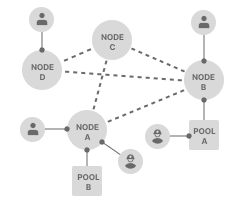
\includegraphics[width=0.8\linewidth]{P2P.png}
    \caption{P2P Encrypted Network, Xelis Team 2024}
    \label{fig:enter-label}
\end{figure}

In this network, seed nodes play a pivotal role by aiding nodes in discovering each other, and these seed nodes are automatically connected when no peer list is available. XELIS employs the ChaCha20-Poly1305 Authenticated Encryption with Associated Data (AEAD) cipher for symmetric encryption, implementing key rotation every 1 GB of data transmitted to enhance security. Data transmission utilizes a custom serializer and deserializer that manually converts data structures into raw bytes based on fixed field positions and bit sizes. This approach ensures efficient and secure data handling.

\subsubsection{Protocol}

The protocol is structured around a packet-based system for data transfer between peers. To establish a connection with a potential peer, the initiating party must first transmit its symmetric encryption key. The receiving party, upon receiving the key, will then send its own encryption key in return. Once both parties have exchanged their symmetric keys, they can proceed with the handshake process and initiate encrypted data transmission.\\

During the handshake, the initiating client sends a handshake packet to the recipient to request an upgrade to a Peer status, to which the recipient responds with a confirmation packet. The handshake packet also allows a peer to indicate whether it consents to sharing its IP address for the purpose of extending peer lists or including it in the RPC API.\\

To optimize bandwidth usage, the protocol mandates that nodes should avoid sending duplicate transactions or blocks to the same peer during propagation. The local node maintains a cache of the most recent N elements sent or received from each peer to prevent redundant transmissions.\\

\subsubsection{Implementation}

For new peer connections, which may be initiated from a queue or through incoming requests, a unique Tokio task with a dedicated buffer is utilized for the handshake process. This design mitigates the risk of Denial of Service (DoS) attacks that could arise from task overload. Once a peer is validated, two distinct tasks are assigned: one for reading incoming packets and another for writing packets. This separation ensures that incoming data does not block outgoing data transmissions.\\

\subsubsection{Chain Synchronization}

Chain synchronization involves the local node randomly selecting a peer with a higher blockchain height and sending a chain request. This request includes the latest block hashes from the local node’s chain, spaced exponentially by their topoheight. The selected peer uses this data to locate a common point between its chain and the local node’s chain. Upon finding a common point, the peer sends back a response with additional block hashes ordered by topoheight. The local node then requests each block data based on the hash list received from the peer to integrate it into its own chain. Chain synchronization requests occur at a minimum interval defined by CHAIN\_SYNC\_DELAY seconds.\\

\subsubsection{Packet Types}
\begin{itemize}
\item \textbf{Key Exchange:} This packet initiates the establishment of an encrypted communication channel by exchanging symmetric encryption keys between peers. The ChaCha20-Poly1305 algorithm is currently used for encryption and decryption. Key rotation occurs every 1 GB of data transmitted, with separate keys employed for encrypting and decrypting packets.

\item \textbf{Handshake:} The handshake packet, which includes blockchain state information, is used to upgrade a connection to Peer status. This packet is sent only at the beginning of a connection and is followed by a response packet from the recipient containing its own blockchain state.\\

\item \textbf{Transaction Propagation:} This packet contains only the transaction hash to avoid duplicating transaction data. A cache per peer tracks previously sent or received transactions to prevent redundancy.\\

\item \textbf{Block Propagation:} This packet includes only the block header and is sent to peers whose blockchain height differs from the local node’s height by less than the STABLE\_LIMIT. Transactions needed to construct the block are retrieved from the mempool, with missing transactions requested from the peer.\\

\item \textbf{Chain Request and Chain Response:} These packet types are used for requesting and responding to chain data, respectively. Details are to be defined.\\

\item \textbf{Ping:} Sent at regular intervals to inform peers of the local node’s blockchain state and potentially include up to MAX\_LEN socket addresses to assist in extending peer lists.\\

\item \textbf{Object Request and Object Response:} Used for requesting using a hash and responding to specific objects. This allows nodes to request blocks / transactions when one is missing.\\

\item \textbf{Notify Inventory Request and Response:} Request the mempool transaction hashes from the peer. This occurs when we’ve finished the chain sync with a peer, or when we’ve connected to a synced peer.\\

\item \textbf{Bootstrap Chain Request / Response:} P2P protocol to sync the top chain state only with all the requirements needed to be fully functional.

\item \textbf{Chain Info:} The chain info contains the chain state (common point, stable height, stable topoheight, stable hash, etc)

\item \textbf {Assets:} retrieve all assets present in the chain

\item \textbf {Keys:} all accounts registered in the chain

\item \textbf {Nonces:} nonce of each account

\item \textbf {Balances:} all balances summary of the accounts for a specific asset

\item \textbf {Balances Details:} all balances details of the accounts for a specific asset

\item \textbf {Blocks metadata:} 80 blocks below stable topoheight containing hash, supply, reward, difficulty, cumulative difficulty, difficulty P variable.

\item \textbf{Disconnect:} This packet is sent when a common peer is disconnected from one of local node peers and is used to update the "propagation map predicate" to maintain synchronization.\\

\end{itemize}\\
This comprehensive design ensures efficient, secure, and resilient communication within the P2P network, supporting a wide range of functionalities and future enhancements.\\

\subsection{XELIS Secure WebSocket for dApps}

XSWD, or XELIS Secure WebSocket for dApps, is a robust protocol designed to securely facilitate data exchange between a wallet and decentralized applications (dApps) using WebSocket technology. Serving as a proxy for the wallet's JSON-RPC API, XSWD ensures that each interaction initiated by a dApp is subject to explicit user authorization. This approach not only enhances security but also provides users with granular control over which functions are executed and what data is accessed, thereby preventing unauthorized access.\\

WebSockets enable real-time, bidirectional communication between web clients and servers, allowing for instant notifications of events related to the wallet. This capability contrasts sharply with traditional methods that might require granting full wallet access to third-party applications. With XSWD, users maintain oversight and control, significantly reducing the risk of unauthorized access.\\

Additionally, XSWD proxies all daemon requests when the wallet is connected to a node, simplifying the development process by allowing developers to manage a single connection while accessing comprehensive blockchain information.\\

\subsubsection{Features and Benefits of XSWD:}

Elimination of RPC Bridge Dependency: XSWD removes the need for additional RPC bridge browser extensions, streamlining the connection process.\\

\begin{itemize}

\item \textbf{Secure dApp Interaction:} It ensures secure connections and authentication with dApps via WebSocket, mitigating risks associated with compromised or malicious applications.\\

\item \textbf{Flexible Permissions:} Users have the ability to grant, deny, or permanently reject dApp requests, offering precise control over data access and interaction.\\

\item \textbf{Ease of Integration:} Integration is simplified through command-line interface (CLI) wallet commands, allowing users to manage the XSWD Server and adjust dApp permissions effortlessly.\\

\item \textbf{Proxy for Daemon Requests:} XSWD functions as a comprehensive proxy, providing a unified API for developers to integrate XELIS into their services or dApps, and maintaining a single connection for all blockchain data.\\

\item \textbf{Real-time Notifications:} Users receive immediate updates on wallet events, such as incoming transactions and new blocks, enhancing responsiveness and awareness.\\

\item \textbf{Standardized Protocol:} Utilizing the WebSocket protocol and JSON-RPC 2.0, XSWD ensures compatibility with a wide range of programming languages and frameworks.\\

\item \textbf{Compatibility:} XSWD is compatible across various platforms and devices, including web browsers, mobile devices, and desktop applications.\\
\end{itemize}
\subsubsection{Protocol Detail:}

The XSWD protocol is built on the WebSocket protocol, with communication conducted using JSON-RPC 2.0. It listens exclusively on port 44325 and the path /XSWD, eliminating the need for configuration on the application side. Upon establishing a connection, the initial message from the application must adhere to the ApplicationData format, which includes fields for a unique application identifier, name, description, URL, permissions, and a signature.\\
\begin{itemize}
  
\item \textbf{id:} A 64-character hexadecimal string uniquely identifying the application.
\item \textbf{name:} A string of up to 32 characters representing the application name.
\item \textbf{description:} A string of up to 255 characters providing a description of the application.
\item \textbf{url:} A valid URL up to 255 characters long, with its origin matching the application's website URL if applicable.
\item \textbf{permissions:} An object detailing user-set permissions, initially empty and updated as permissions are granted or denied.
\item \textbf{signature:} A hexadecimal string generated by the wallet to validate the permissions, signed over the hash of the ApplicationData fields (excluding the signature field itself).\\
d{itemize}
\end{itemize}
Upon a successful request, XSWD responds with a confirmation message. In case of failure, it provides an error message in JSON-RPC format detailing the issue using JSON format.\\

\subsubsection{Permissions Management:}

Permissions in XSWD are defined based on the RPC method requested:\\

\begin{itemize}
\item \textbf{ask:} The application must request permission from the user for each action.


\item \textbf{accept\_always:} The application is granted permission to execute the request without further user approval.

\item \textbf{deny\_always:} The application is permanently denied permission, with no further prompts to the user until permissions are modified.
Permissions are session-specific and not persisted within the wallet; applications must store and manage permissions independently if persistence is required.
\end{itemize}
This structured approach ensures a high level of security, flexibility, and ease of use for interactions between wallets and decentralized applications.

\subsubsection{RPC Methods:}\\

XSWD leverages the same RPC methods as the JSON-RPC API of the wallet, with a crucial distinction: RPC methods intended for the wallet must be prefixed with wallet.. This ensures that all requests are correctly routed to the wallet component. For a comprehensive list of these methods, please refer to the JSON-RPC API documentation.\\

Similarly, methods destined for the daemon should be prefixed with node. It is important to note that RPC methods prefixed with node are only accessible when the wallet is connected to a node and do not require user-set permissions. This design allows for seamless integration and interaction with the daemon without additional authorization steps.\\

In addition to these RPC methods, XSWD also supports listening to any wallet events traditionally available through the RPC API, thereby maintaining full functionality and real-time event handling.

\subsubsection{Future Features}

Looking ahead, we are exploring several enhancements to XSWD to increase its versatility and security:\\

\begin{itemize}
\item \textbf{Multi-Wallet Proxy System:} Currently, XSWD supports a single instance per device. We are developing a proxy system that will enable the distribution of requests across multiple wallets. This feature will benefit advanced users who manage several wallets simultaneously and developers who need to test their applications across multiple wallet instances. This capability will provide a more flexible and scalable solution for managing diverse wallet interactions.

\item \textbf{TLS Support with Randomly Generated Certificates:} To further secure communication between applications and the wallet, we are considering implementing TLS support with randomly generated certificates. This enhancement aims to bolster the security of WebSocket communications. However, it is important to note that self-signed certificates are not supported by standard web browsers, which may limit compatibility. Therefore, this feature may be reserved for specific applications or environments where enhanced security is essential.\\
\end{itemize}
These forthcoming features are designed to extend the functionality and security of XSWD, providing users and developers with advanced tools for managing and securing their blockchain interactions.

\subsection{Smart Contracts}

Smart Contracts are an innovative feature designed to facilitate the automation and secure execution of contractual agreements directly on the blockchain. Utilizing a bespoke interpreted language within a dedicated Virtual Machine, these contracts eliminate the need for intermediaries by embedding the terms of the agreement into executable code. This approach ensures that contracts are enforced transparently and reliably, executing automatically when predefined conditions are met.

Smart Contracts have a wide range of potential applications, including but not limited to:\\

\begin{itemize}
\item \textbf{Decentralized Applications (dApps):} Enabling the creation of applications that run on a decentralized network without a central authority.

\item \textbf{Tokenization of Assets:} Facilitating the representation of physical or digital assets as tokens on the blockchain.

\item \textbf{Voting Systems:} Implementing secure and verifiable voting mechanisms.

\item \textbf{Supply Chain Management:} Enhancing transparency and traceability throughout supply chains.\\
\end{itemize}

Currently, Smart Contracts are not yet available on the XELIS mainnet but are slated for future implementation with a testnet expected shortly. The XELIS coin is designed as the utility token for all transactions and fees within the XELIS ecosystem, including smart contracts and decentralized applications (dApps). As the native currency, XELIS will be used to pay for transaction fees, smart contract execution, and interactions within dApps, ensuring a seamless and integrated user experience. By leveraging XELIS as a universal medium for these operations, the ecosystem ensures efficient and secure processing of various functions while maintaining a cohesive economic model that supports the growth and sustainability of both the blockchain and its associated applications.

\subsection{XELIS Virtual Machine (XVM)}

The XELIS Virtual Machine (XVM) is an advanced execution environment specifically designed for the XELIS network, utilizing an interpreted language developed in Rust. The XVM supports a comprehensive set of programming constructs, including constants, functions, while and foreach loops, arrays, and structures. Its syntax draws heavily from Rust and Go languages, offering a robust and familiar programming environment.\\

\subsubsection{Key features of the XVM include:}

\textbf{Parser Verification:} Code is verified primarily at the parsing stage to ensure compliance with the syntactic and semantic rules of the language.\\

\textbf{Primitive Types:} The language supports several primitive types, including:
u8 (Unsigned 8-bit integer),
u16 (Unsigned 16-bit integer),
u32 (Unsigned 32-bit integer),
u64 (Unsigned 64-bit integer),
u128 (Unsigned 128-bit integer),
bool (Boolean),
string (String),
struct (Structure),
optional<T> (Nullable type where T is another data type),\\

Files written for the XVM are saved with the .xel extension. For additional information and to access the complete documentation, please follow the provided link to the XVM documentation. https://docs.xelis.io/features/smart-contracts 

\subsection{Confidential Assets}

Confidential Assets are a unique feature allowing anyone to create its own asset / token and be fully compatible with wallets, exchanges and other services supporting XELIS. This is possible because it is directly implemented on the base layer of the blockchain, and not as a second layer solution.\\

Each asset is represented by a unique asset ID (32 bytes hash). This asset ID is used to identify the asset in transactions and in the blockchain.It allows to have fully private balances and transferred amounts just like XELIS. As an example, XELIS is a confidential asset itself with the asset ID 00000000000000..............000000000000000.\\

\subsubsection{Advantages of Confidential Assets}
\begin{itemize}
\item \textbf{Privacy:} Confidential Assets allow to have fully private balances and transferred amounts.\\

\item \textbf{Compatibility:} Confidential Assets are fully compatible with wallets, exchanges and other services.\\

\item \textbf{Security:} Confidential Assets are implemented on the base layer 1 of the blockchain, and not as a second layer solution.\\

\item \textbf{Decentralized:} Confidential Assets are fully decentralized and trustless, nobody can freeze or censor your assets.\\

\item \textbf{Management:} if deployed by a Smart Contract, the Confidential Asset can be managed by the owner for specific properties/tokenomics(ie. A stablecoin with mint/burn mechanism). Confidential assets deployed outside of a Smart Contract cannot be managed by the owner. This means that the owner cannot mint or burn the assets you own, but also cannot take, for example, a \% fee on each transfer.\\
\end{itemize}

\section{Economics of the Protocol and XELIS Coin}

The current consensus configuration is as follows:

\begin{itemize}
    \item Target Block Time: 15 seconds.
    \item Minimum Transaction Fee: 0.00001000 XEL per kilobyte (KB).
    \item Decimal Precision: The full coin can be subdivided into up to 8 decimal places.
    \item Maximum Supply: Capped at 18.4 million coins.
    \item Maximum Block Size: Limited to 1.25 megabytes (MB).
    \item Maximum Transaction Size: Restricted to 1 megabyte (MB).
    \item Address Prefixing: To prevent address conflicts across different networks, addresses are prefixed accordingly. Mainnet addresses start with "xel," while addresses for the development and test networks begin with "xet."
\end{itemize}


\subsection{Mining Reward and Supply Emission}\\

The mining reward is how the XELIS supply is introduced into circulation. This mechanism not only incentivizes miners to secure and validate transactions but also dictates how much supply is circulating.\\

In the XELIS network, the initial mining reward is set at approximately 1.41 XEL per block. Unlike traditional cryptocurrencies that utilize a halving structure—where the block reward is reduced by 50\% at regular intervals—our system implements a gradual decrease in reward based on a supply and emission factor of 20 similar to Monero. Instead of a sharp, predetermined reduction, this method ensures a more stable and predictable decrease in rewards over time.\\

The reward adjustment in our network is distinct from the halving model in several ways. In traditional halving models, the reward reduction is fixed and occurs at set intervals, leading to predictable but occasionally abrupt changes in miner incentives. In contrast, our emission model allows for a more nuanced adjustment of rewards that reflects the overall supply dynamics.\\

\begin{figure}
    \centering
    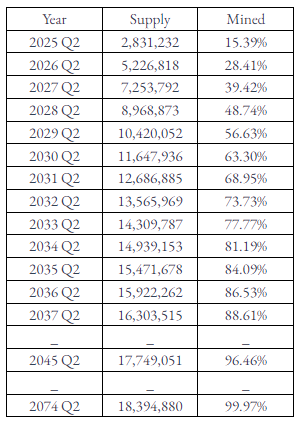
\includegraphics[width=0.7\linewidth]{Screenshot 2024-10-23 185252.png}
    \caption{XELIS Emission Schedule}
    \label{fig:enter-label}
\end{figure}

Additionally, the actual reward received by miners can be impacted by network conditions, such as the presence of side blocks—alternative blocks mined at the same height. The reward may be adjusted downward, ranging from a minimum of 5\% to a maximum of 30\% of the initial reward, depending on the number of side blocks encountered. This configuration guarantees that miners of side blocks are also fairly compensated. Such variability stems from the inherent characteristics of the Directed Acyclic Graph (DAG) and the competitive nature of the mining environment.


\subsection{Maximum Supply}
XELIS is designed with a capped maximum supply of 18.4 million XEL, a limit that will be gradually approached over an extended period of 50 years. This fixed maximum supply is a fundamental aspect of the XELIS economic model, ensuring long-term scarcity and value stability for the cryptocurrency. The supply emission schedule is carefully structured to achieve this cap, with the total number of XEL gradually increasing as new blocks are mined. This gradual approach not only contributes to the stability of the currency but also aligns with the long-term vision of maintaining a predictable and controlled inflation rate. The 50-year timeline for reaching the maximum supply is intended to create a balanced and sustainable economic environment for miners and holders of XEL throughout the cryptocurrency's emission schedule.
\subsection{Miner Development Fee}

XELIS operates as a community-driven initiative, independent of any corporate or organizational backing. To support its development, ensure its ongoing success, and provide sustained assistance, we have implemented a dynamic development fee structure. This fee begins at 10\% of the block reward and is designed to decrease over time. This funding mechanism is essential for establishing a robust initial ecosystem, guaranteeing a continuous flow of capital dedicated exclusively to the growth and advancement of the blockchain.\\

The development funds are allocated strictly for network development expenses and adoption expenses, and are not intended for personal gain or market manipulation. The community plays a vital role in overseeing these funds, with opportunities to suggest, inquire about, and influence how they are utilized.\\

The development fee schedule is as follows:

\begin{itemize}
    \item 10\% from block 0 to 3,249,999 (approximately the first 1.5 years with BlockDAG)
    \item 5\% from block 3,250,000 onwards, until the project achieves stability in key aspects of the ecosystem as decided upon by the development team. \end{itemize}
This gradual reduction in the development fee serves multiple purposes. One key objective is to prevent early, large-scale miners from disproportionately benefiting during the initial phases of the project, when block rewards are at their highest and mining difficulty is relatively low. This measure helps to mitigate the risk of rapid accumulation and potential market manipulation by a few entities. Despite this, miners will still have ample opportunities to earn profits and reinvest as they see fit.\\

\textit{Long Term Vision for Development Fee:} Ideas of creating a DAO to manage the funds, reducing, or even simply removing the dev fees are currently in discussion. \\

In summary, the development fee is a well-considered solution to address the challenges of maintaining and growing the XELIS platform. The funds are crucial for fostering a healthy and evolving ecosystem, and to eliminate needing to rely on community donations which can be inconsistent, and lead to individuals who donate substantial amounts of money, exerting disproportionate influence over the project's direction, governance, and decision-making processes. The goal is to ensure that the funds are used to benefit the network and maintain a level playing field, rather than serving the interests of powerful entities seeking short-term gains.


\section{Team and Community Contributors}

The XELIS core team is composed of experienced developers from the blockchain and technology sectors. While individual identities have not been publicly disclosed, the collective expertise and substantial contributions to various projects highlight the team's capability and commitment to XELIS's success. The track record of contributions can be seen on the developers' GitHub and Stack Overflow profiles.\\

In addition to the core team, several community contributors have donated time in various aspects of development, business development, marketing, content creation, community building, and developing partnerships. 

\subsection{Privacy and Future Disclosure of Team Identities}

At this time, the identities of the core team and community contributors have not been disclosed to the public. This approach maintains a focus on the project’s development and objectives rather than personal profiles. The priority is to build a high-quality product that effectively addresses user needs and drives the initiative's success.\\

Transparency is recognized as crucial for establishing trust within the community and the broader industry. As the project evolves and reaches significant milestones, there is consideration of the potential for revealing identities. This future disclosure aims to further solidify commitment and foster a stronger connection with stakeholders.

\subsection{Community Involvement}
In addition to the core team, XELIS thrives on community engagement, encouraging everyone to contribute to its development, marketing, and community initiatives. All participants who take part through the ‘proof of participation’ ethos will be warmly welcomed.

\section{Legal Considerations}\\
\begin{itemize}
\item \textbf{General Information}\\

The information provided in connection with XELIS (the "Project") is for informational purposes only and does not constitute financial, investment, legal, or professional advice. XELIS is a cryptocurrency project and operates within the blockchain ecosystem, which is subject to various risks and regulatory uncertainties. Participation in the Project, including the purchase, sale, or use of XELIS coins, involves a high degree of risk and may not be suitable for all individuals.\\

\item \textbf{No Offer or Solicitation}\\

Nothing contained in this document constitutes an offer or solicitation to buy or sell any securities, financial products, or services, nor does it constitute investment advice. The XELIS coins and related activities are not offered or intended to be sold to, or used by, individuals in any jurisdiction where such offer, solicitation, purchase, or use would be unlawful under applicable law.\\

\item \textbf{Regulatory Status}\\

The regulatory status of cryptocurrencies and related activities varies by jurisdiction and is continually evolving. XELIS makes no representations or warranties regarding the regulatory status or compliance of the Project, XELIS coins, or any related activities. Participants are solely responsible for ensuring compliance with all applicable laws and regulations in their respective jurisdictions. XELIS has not yet obtained a legal opinion, but does have future plans to obtain this. \\

\item \textbf{Risks}\\

Participation in the XELIS Project involves significant risks, including but not limited to, the risk of loss of capital, volatility in the value of XELIS coins, technological risks, security risks, and regulatory risks. The value of cryptocurrencies can fluctuate widely and is subject to various factors beyond the control of XELIS. Potential participants should conduct their own due diligence and consult with financial, legal, and tax professionals before participating in the Project.\\

\item \textbf{No Guarantees}\\

XELIS makes no representations or warranties of any kind, express or implied, regarding the future performance or value of XELIS coins. There is no guarantee that XELIS will achieve its goals or that XELIS coins will have any value. Past performance is not indicative of future results.\\

\item \textbf{Limitation of Liability}\\

To the maximum extent permitted by law, XELIS, its team, community, and affiliates,shall not be liable for any direct, indirect, incidental, consequential, special, or punitive damages arising from or in connection with the Project, the use or inability to use XELIS coins, or any reliance on information provided by XELIS.\\

\item \textbf{Changes and Updates}\\

XELIS reserves the right to modify or update this disclaimer at any time without prior notice. Participants are encouraged to review this disclaimer periodically for any changes. 
\end{itemize}

 \section{Conclusion}
 
The quadlemma framework of decentralization, security, scalability, and privacy marks a new frontier in blockchain development. Each of these four pillars is vital for building a robust cryptocurrency ecosystem, but achieving an optimal balance is incredibly challenging. Some blockchains may focus on specific use cases that require more emphasis on privacy (such as financial confidentiality), while others may prioritize scalability for mass adoption (e.g., payment platforms).\\

The quadlemma highlights the inevitable compromises that come with blockchain design:

\begin{itemize}
    \item \textbf{A privacy-focused blockchain may struggle with scalability and decentralization.}
    \item \textbf{A highly scalable blockchain might sacrifice privacy and decentralization.}
    \item \textbf{Decentralized blockchains, like Bitcoin, might prioritize security but lack scalability and privacy.}
\end{itemize}

XELIS approaches each of the four pillars uniquely and provides direct solutions to solve the cryptocurrency Quadlemma.\\


    \subsection{Decentralization in XELIS}\\

Decentralization is one of the most critical aspects of any blockchain system, as it ensures the network remains open, censorship-resistant, and free from centralized control. XELIS employs a Proof-of-Work (PoW) consensus mechanism to secure decentralization. PoW, in which miners validate transactions by solving complex mathematical problems, has a proven track record of promoting decentralization, as seen in Bitcoin and other early cryptocurrencies.\\

However, unlike Bitcoin, which has seen mining centralization due to the rise of specialized hardware (ASICs), XELIS uses an ASIC-resistant PoW algorithm (and FPGA-resistant) designed to democratize mining. By resisting ASIC dominance, XELIS ensures that mining can be performed using general-purpose hardware, such as GPUs and CPUs, which opens participation to a broader base of users. This prevents mining power from becoming concentrated in a small number of industrialized mining farms and keeps the network decentralized.\\

XELIS' emphasis on GPU's and CPU's co-existing on one algorithm reduces the risk of centralization and keeps control of the network distributed across a wide number of miners, promoting fairness and making it difficult for any single entity to dominate the mining process.\\

\subsection{Security in XELIS}\\

Security is paramount for any cryptocurrency, as vulnerabilities in the system can lead to theft, double-spending, or other forms of attack. XELIS leverages its PoW consensus mechanism along with its BlockDAG to maintain a high level of network security, ensuring that any malicious attempt to alter the blockchain would require immense computational power, making attacks economically unfeasible.\\

By ensuring a wide distribution of miners due to its ASIC resistance, XELIS reduces the risk of any single entity gaining sufficient mining power to attack the network. Additionally, the design of the PoW algorithm encourages consistent participation and competition among miners, further reinforcing the network's security.\\

Furthermore, XELIS takes advantage of its homomorphic encryption cryptographic technology to bolster the security of individual transactions. XELIS' Homomorphic encryption allows transactions to be transmitted without revealing transferred amounts and wallet balances. This adds an additional layer of anonymity and protection against tracking large wallet balances and transactions from external parties who might leverage this information in attempting fraudulent activities.\\


\subsection{Scalability in XELIS}\\

Scalability is one of the greatest challenges in blockchain, particularly for PoW-based networks that typically prioritize security and decentralization over transaction throughput. XELIS addresses this by adopting a blockDAG architecture and optimized transaction validation process, allowing it to process more blocks and transactions per second (TPS) compared to traditional PoW networks like Bitcoin.\\

XELIS improves scalability in the following ways:
\begin{itemize}
    \item \textbf{Efficient Block Size:} XELIS implements a maximum 1.25MB block size. This block size, combined with our 15 second block time on a BlockDAG architecture, ensures that the network can handle higher transaction volumes without experiencing significant slowdowns or congestion.
    \item \textbf{Fast Transaction Finality:} XELIS' block times and blockDAG architecture are optimized to ensure faster confirmation times for transactions, which improves the overall throughput of the network. This makes XELIS more suitable for everyday payments and micro-transactions compared to slower PoW networks, which often struggle with high confirmation times.
\end{itemize}

By leveraging these techniques, XELIS ensures that the network can scale effectively while still maintaining its core principles of decentralization and security. Unlike blockchains that require layer-2 solutions or centralized shortcuts or indexers to increase scalability, XELIS focuses on optimizing its base layer to handle higher transaction volumes without sacrificing decentralization or security.\\


\subsection{Privacy in XELIS}\\

Privacy is a critical concern for many cryptocurrency users, especially in an era where blockchain analytics are becoming more sophisticated and invasive. In addition, privacy must also be balanced, providing the correct amount of privacy for users to keep their financial histories safe, but complying with modern day governmental regulations and stipulations.\\

XELIS prioritizes privacy by integrating the first ever partial privacy scheme. Utilizing Homomorphic Encryption and Zero Knowledge Proofs, these features ensure that sender and receiver addresses remain public, but the transaction amounts and wallet balances are obfuscated from the public.\\


Here's how these privacy features work:
\begin{itemize}
    \item \textbf{Homomorphic Encryption:} Homomorphic Encryption (HE) enhances privacy by allowing computations on encrypted data without requiring decryption, ensuring that sensitive information remains confidential throughout the process. In the XELIS ecosystem, this cryptographic method, particularly through the ElGamal encryption system, is used to protect transaction details such as account balances and transfer amounts. XELIS employs a variant known as Twisted ElGamal over Ristretto Points, which integrates Pedersen commitments to work seamlessly with Bulletproofs, ensuring efficient transaction verification while retaining strong security. The homomorphic properties of ElGamal, specifically its additive and subtractive capabilities, allow for secure balance adjustments on the blockchain without exposing sensitive data.

    \item \textbf{Zero-Knowledge Proofs:} Zero-Knowledge Proofs (ZKPs) are a cryptographic technique that enables one party (the prover) to demonstrate knowledge of certain information to another party (the verifier) without revealing the information itself. In XELIS, ZKPs are crucial for validating encrypted transactions, ensuring that the amount being transferred is correct without revealing sensitive details. Specifically, XELIS employs Bulletproofs, a non-interactive ZKP protocol, to verify that transferred amounts are within valid ranges and non-negative, ensuring transaction integrity. XELIS further optimizes Bulletproofs with batching, aggregation, and source commitments, leading to rapid transaction verification times. These optimizations allow XELIS to process up to 2,500 transactions per second, while also addressing challenges like front-running and maintaining transaction order in a scalable BlockDAG architecture.
\end{itemize}

These privacy features are built directly into the core of XELIS, rather than being optional add-ons, making the network inherently privacy-preserving. Having them embedded directly into the core Layer-1 protocol allows XELIS' soon-to-be launched Smart Contracts, Virtual Machine, and Defi Applications and Assets to retain these privacy features.\\

In conclusion, XELIS is focused on advancing blockchain technology through its innovative solution to solve the quadlemma by a combination of BlockDAG architecture, advanced cryptographic methods, and account-based model. The platform tackles the important challenge of balancing transparency and privacy, ensuring that user data remains secure while still enabling necessary oversight and regulatory compliance. By utilizing homomorphic encryption and a streamlined ledger system, XELIS aims to provide scalability, speed, and flexibility, supporting confidential transactions and the development of decentralized applications.\\

With a commitment to enhancing user privacy and implementing robust security measures, XELIS positions itself as a viable solution in the evolving digital landscape. As the ecosystem continues to grow, the goal is to create an environment where users can interact, transact, and innovate with confidence, knowing their data is protected and their experience is smooth. XELIS is prepared to meet the demands of the next generation of digital interactions, prioritizing security, privacy, and efficiency in blockchain technology.\\

\newpage
~\newpage

\section{References}

Atzori, M. (2017). Blockchain Technology and Decentralized Governance: is the State Still Necessary? Journal of Governance and Regulation, 6(1), 45-62. https://dx.doi.org/10.22495/jgr\_v6\_i1\_p5 \\

BLAKE3. BLAKE3: The next-generation cryptographic hash function. Available from Blake3 Github: https://blake3.io/\\

Böhme R, Christin N, Edelman B, Moore T. Bitcoin: Economics, technology, and governance. J Econ Perspect. 2015;29(2):213-238. doi:10.1257/jep.29.2.213.\\

Bowe, A, Gikay, R, and Mowery, C. The Monero Research Lab. Monero: A Secure, Private, and Untraceable Cryptocurrency. 2014. Available from: https://www.getmonero.org/resources/ research-lab/monero.pdf \\

Bootle J, Bünz B, Boneh D, Maxwell G, Poelstra A, Wuille P. Bulletproofs: Short Proofs for Confidential Transactions and More. In: 2018 IEEE Symposium on Security and Privacy (SP). San Francisco, CA: IEEE; 2018:315-334. DOI:10.1109/SP.2018.00020.\\

Buterin V. A Next-Generation Smart Contract and Decentralized Application Platform. Ethereum White Paper. 2013. Available from: https://ethereum.org/en/whitepaper/\\

Chen T, Li H, Zhang X, et al. An Overview of Blockchain Technology: Architecture, Consensus, and Future Trends. IEEE Access. 2019;7:170075-170088. doi:10.1109/ACCESS.2019.2957479.\\

Chen, Y., Ma, X., Tang, C., and Au, M. H. Pgc: Decentralized confidential payment system with auditability. In European Symposium on Research in Computer Security (2020), Springer, pp. 591–610.\\

Cramer R, Damgård I, Schoenmakers B. Proofs of Partial Knowledge and Simplified Design of Witness Hiding Protocols. In: CRYPTO '94: Proceedings of the 14th Annual International Cryptology Conference on Advances in Cryptology. Santa Barbara, CA: Springer-Verlag; 1994:174-187. DOI:10.1007/3\-540-48658-5\_18.\\

Decker C, Wattenhofer R. Information Propagation in the Bitcoin Network. In: Proceedings of the 13th IEEE International Conference on Peer-to-Peer Computing. Trento, Italy: IEEE; 2013:1-10. DOI:10.1109/P2P.2013.6688704.\\

Diffie W, Hellman M. New Directions in Cryptography. IEEE Trans Inf Theory. 1976;22(6):644-654. doi:10.1109/TIT.1976.1055638.\\

Elgamal T. A Public Key Cryptosystem and a Signature Scheme Based on Discrete Logarithms. IEEE Trans Inf Theory. 1985;31(4):469-472. DOI:10.1109/TIT.1985.1057074.\\

Garay J, Kiayias A, Leonardos N. The Bitcoin Backbone Protocol: Analysis and Applications. In: Proceedings of the 2015 IEEE European Symposium on Security and Privacy (EuroS\&P); 2015: 105-120. doi:10.1109/EuroSP.2015.26.\\

Gentry C. Fully Homomorphic Encryption Using Ideal Lattices. In: Proceedings of the 41st Annual ACM Symposium on Theory of Computing (STOC). Bethesda, MD: ACM; 2009:169-178. DOI:10.1145/1536414.1536440.\\

Goldwasser S, Micali S, Rackoff C. The Knowledge Complexity of Interactive Proof-Systems. SIAM J Comput. 1989;18(1):186-208. DOI:10.1137/0218012.\\

Goldwasser S, Micali S, Rackoff C. The knowledge complexity of interactive proof systems. SIAM J Comput. 1989;18(1):186-208. doi:10.1137/S0097539791191349.\\

Horizen Academy. UTXO vs Account Model. Available from: https://www.horizen.io/academy/utxo-vs-account-model/ \\

Kiayias A, Tselekounis Y, Zindros D. Non-interactive proofs of proof-of-work. In: 2020 IEEE European Symposium on Security and Privacy (EuroS\&P). London, UK: IEEE; 2020:282-297. doi:10.1109/EuroSP48018.2020.00032.\\

Krause M, Tolaymat T. Quantifying the Energy and Carbon Costs of Bitcoin Mining. Nat Commun. 2018;9(1):1-7. doi:10.1038/s41467-018-03040-4.\\

Krolikowski D, Saito Y, Sato Y, et al. BLAKE3: A Fast and Secure Hash Function. 2020. Available from: https://eprint.iacr.org/2020/769.pdf\\

Kurose JF, Ross KW. Computer Networking: A Top-Down Approach. 8th ed. Boston, MA: Pearson; 2018.\\

Liu, Y., and Zhang, J. Evaluating Monero: A Privacy-focused Cryptocurrency. In: Proceedings of the 2019 IEEE International Conference on Blockchain; 2019: 1-8. doi:10.1109/Blockchain.2019.00014.\\

Lovecruft, I. A., and de Valence, H. curve25519-dalek. https://github.com/dalek-cryptography/curve25519-dalek, 2021.\\

Luu L, Chu D, Olickel H, et al. A Secure Sharding Protocol for Open Blockchains. In: Proceedings of the 2016 ACM SIGSAC Conference on Computer and Communications Security; 2016:17-30. doi:10.1145/2976749.2978303.\\

Mowery, C. An Overview of Monero's Privacy Mechanisms: Ring Signatures, Stealth Addresses, and RingCT. In: Proceedings of the 2017 IEEE European Symposium on Security and Privacy (EuroS\&P); 2017: 163-178. doi:10.1109/EuroSP.2017.43.\\

Mougayar W. The Business Blockchain: Promise, Practice, and the Application of the Next Internet Technology. Wiley; 2016.\\

Nakamoto S. Bitcoin: A Peer-to-Peer Electronic Cash System. 2008. Available from: https://cdn.nakamotoinstitute.org/docs/ bitcoin.pdf \\

National Institute of Standards and Technology. NIST Special Publication 800-185: The BLAKE Hash Function. 2015. Available from: https://nvlpubs.nist.gov/nistpubs/ SpecialPublications/NIST.SP.800-185.pdf \\

Noether, S. Proof-of-Work and the Blockchain. Monero Research Lab. 2015. Available from: https://www.getmonero.org/resources/
research-lab/monero-proof-of-work.pdf \\

Pedersen T. Non-Interactive and Information-Theoretic Secure Verifiable Secret Sharing. In: Goldwasser S, editor. Advances in Cryptology – Crypto’91. Lecture Notes in Computer Science. Vol 576. Berlin, Heidelberg: Springer; 1992:129-140. DOI:10.1007/3-540-46766-1\_9.\\

Preneel B, Van Oorschot PC. Cryptographic Hash Functions: A Survey. In: Cryptography and Security: Principles and Practice. New York, NY: Springer; 2003:137-166. doi:10.1007/978-1-4757-3346-4\_7.\\

Rhea SY, Godfrey PC, Manku GS, et al. OpenDHT: A Public DHT Service and its Applications. In: Proceedings of the 2005 USENIX Annual Technical Conference; 2005:49-64.\\

Twisted ElGamal. Solana. Available from: https://spl.solana.com/assets/files/ twisted\_elgamal-2115c6b1e6c62a2bb4516 891b8ae9ee0.pdf\\

Schnorr CL. Efficient Identification and Signatures for Smart Cards. In: CRYPTO '89: Proceedings of the 9th Annual International Cryptology Conference on Advances in Cryptology. Santa Barbara, CA: Springer-Verlag; 1990:239-252. DOI:10.1007/0-387-34805-0\_22.\\

Singh R, Srivastava G, Dhar Dwivedi A. PHANTOM Protocol as the New Crypto-Democracy. In: Saeed K, Homenda W, editors. Computer Information Systems and Industrial Management: 17th International Conference, CISIM 2018. Vol 11127. Olomouc, Czech Republic: Springer; 2018. p. 499-509. DOI:10.1007/978-3-319-99954-8\_41.\\

Smart NP, Zhang L. Solving Small Exponential ECDLP in EC-based Additively Homomorphic Encryption and Applications. IACR Cryptol ePrint Arch. 2022:1573. Available from: https://eprint.iacr.org/2022/1573\\

Szabo N. Smart Contracts: Building Blocks for Digital Markets. First Monday. 1997;2(9). doi:10.5210/fm.v2i9.548.\\

Szabo N. The Idea of Smart Contracts. First Monday. 1997;2(9). doi:10.5210/fm.v2i9.548.\\

Tanenbaum AS, Wetherall D. Computer Networking. 5th ed. Boston, MA: Pearson; 2011.\\

Voshmgir S. Tokenomics: Dynamic Adoption and Valuation. 1st ed. Berlin, Germany: BlockchainHub; 2020.\\

Waghmare D, Ghosh R. Blockchain and DAG: An Overview. In: Proceedings of the 2020 4th International Conference on Cloud Computing and Blockchain Technology. Paris, France: IEEE; 2020:18-23. doi:10.1109/CCBT49710.2020.00007.\\

Wang Y, Li Q, Jiang X, et al. A Survey on Smart Contracts: Challenges and Opportunities. IEEE Access. 2020;8:131417-131431. doi:10.1109/ACCESS.2020.3002915.\\

Xu X, Weber I, Staples M. Architecture for Blockchain Applications. Berlin, Germany: Springer; 2019.\\

Zhang J, Wang S, Wang Y, et al. Performance Evaluation of Cryptographic Hash Functions. In: 2019 IEEE International Conference on Computing, Networking and Communications (ICNC); 2019:246-250. doi:10.1109/ICCNC.2019.8685528.\\

Zhang S, Zhao C, Zhang H, et al. A Survey on DAG-based Blockchain: Concepts, Applications, and Future Directions. IEEE Access. 2020;8:94888-94905. doi:10.1109/ACCESS.2020.2996686.\\

Zohar A, Sompolinsky Y. Secure High-Rate Transaction Processing in Bitcoin. In: Proceedings of the 19th International Conference on Financial Cryptography and Data Security (FC). Puerto Rico: Springer; 2015:507-527. DOI:10.1007/978-3-662-47854-7\_32.\\





\end{document}
